\section{Datasets}
\label{sec:db}

The annotated segmentation and saliency datasets, which are used by the researchers to test the algorithms are often made available to the object saliency detection and segmentation community.

\subsection{Saliency Datasets}
\subsubsection{MSRA}
The MSRA  Database form the Visual computing group of Microsoft  research \cite{msra_db} is a collection of two image sets. The first set consists of $20 000$ images labeled by three users, while the second set consists of $5000$ images labeled by nine users. The labeling are available as bounding boxes. Figure \ref{fig:msra} illustrates the dataset.
\begin{figure}[H]
\begin{center}
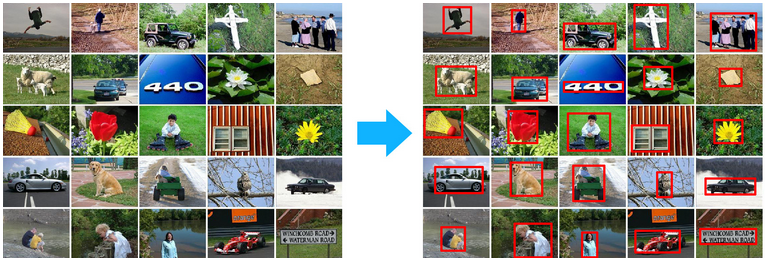
\includegraphics[width=0.95\textwidth]{fig/MSRA}
\end{center}
\caption{Examples of the MSRA dataset.}
\label{fig:msra}
\end{figure}
\subsubsection{MSRA10k}
This is an extension of the MSRA dataset, which  addresses the coarse-grained limitation of the MSRA labeling (bounding boxes). The MSRA10k (\cite{msra10k_db}) dataset consists of $10000$ randomly selected MSRA images for which a pixel-level saliency labeling is available. Figure \ref{fig:msra10k} illustrates the dataset. 
\begin{figure}[H]
\begin{center}
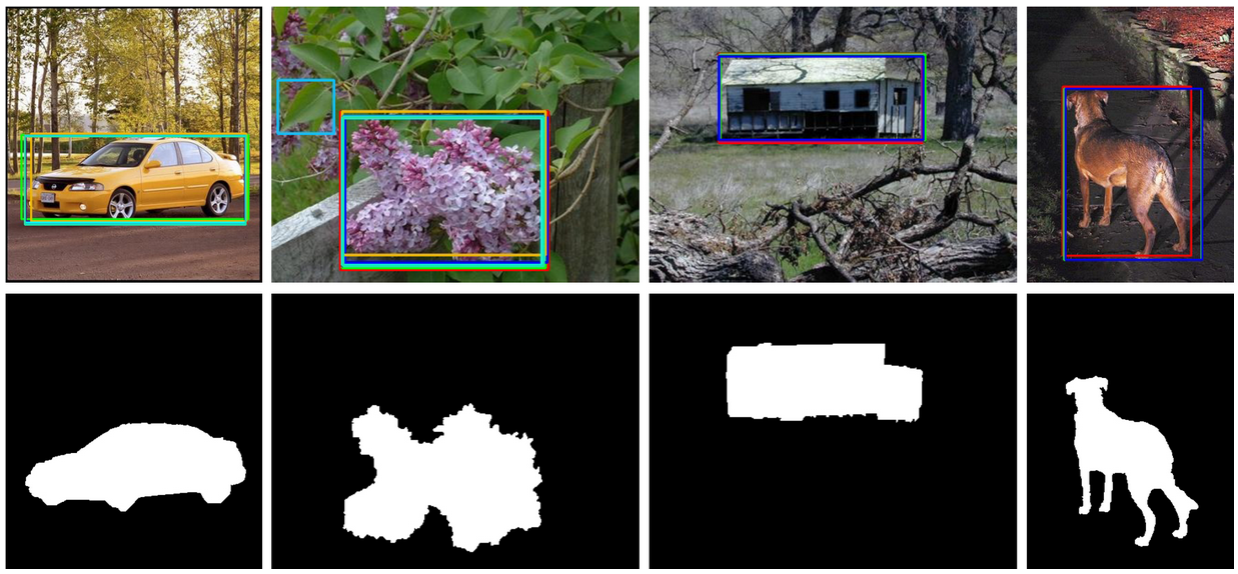
\includegraphics[width=0.95\textwidth]{fig/MSRA10k}
\end{center}
\caption{Examples of the MSRA 10k dataset. First row: original images with ground truth rectangles from MSRA dataset. Second row: Ground truth with pixel accuracy.}
\label{fig:msra10k}
\end{figure}
This dataset is used by in a very recent paper in IEEE Transactions on PAMI \cite{ChengPAMI2015} and \cite{chengPAMIUrl} (online resources with link to the software). 

\subsubsection{CSSD and ECSSD}
Although images from MSRA-1000 \cite{LCAV-CONF-2009-012} have a large variety in their content, background structures are primarily simple and smooth. To represent the situations that natural images generally fall into, the Complex Scene Saliency Dataset (CSSD) \cite{cssd_db} was proposed in \cite{YanCVPR2013} with $200$ images. They contain diverse patterns in both foreground and background. The labeling has done by five  helpers. These images were collected from the BSD300 (later extended to BSD500, \cite{bsd300/500_db}), VOC dataset \cite{voc_db} and internet.

Later, the CSSD was extended to a larger dataset (ECSSD) of $1000$ images, which includes many semantically meaningful and structurally complex images for evaluation. The images are acquired from the internet and five helpers were asked to produce the ground truth masks. Examples of the images in the dataset can be seen on Figure \ref{fig:ecssd}.

\begin{figure}[h]
\begin{center}
\includegraphics[width=0.95\textwidth]{fig/ECSSD}
\end{center}
\caption{Examples of the ECSSD dataset.}
\label{fig:ecssd}
\end{figure}

\subsection{DUT-OMRON}
The datasets mentioned so far, although widely used in the community are not {\em large-scale} per se. The Dalian University of Technology and the Omron Corporation introduced in the DUT-OMRON dataset \cite{dut-omron_db} consisting of $5168$, manually selected from more than $140 000$ images. They are re-sized to $400 \times x$ or $x \times 400$, where  $x < 400$. They contain one or more salient objects with relatively complex background. Five people have labeled the pixel-wise ground truth along with bounding box and eye-fixation. The dataset is illustrated on Figure \ref{fig:dut-omron}. The results of the experiments on the collected dataset were published in \cite{yang2013saliency}.

\begin{figure}[h]
\begin{center}
\includegraphics[width=0.75\textwidth]{fig/DUT-OMRON}
\end{center}
\caption{Samples of the DUT-OMRON dataset.From top to bottom: original image, bounding box ground truth, pixel-wise ground truth,average of the five binary masks and eye-fixation ground truth. }
\label{fig:dut-omron}
\end{figure}

\subsection{PASCAL-S}
Another dataset, which aims at bridging the gap between fixations and salient objects is the PASCAL-S dataset \cite{pascal-s_db} provided by Georgia Tech, Caltech and UCLA. The dataset contains $850$ images from the PASCAL 2010 with $12$ subjects and $1296$ object instances. The images and the code are available for download. The dataset is is illustrated on Figure \ref{fig:pascal-s}.

\begin{figure}[H]
\begin{center}
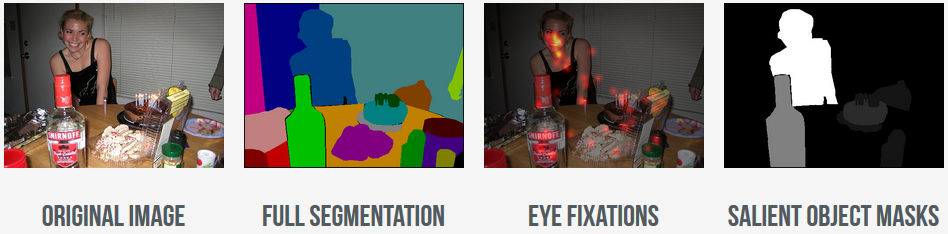
\includegraphics[width=0.95\textwidth]{fig/PASCAL-S}
\end{center}
\caption{Examples of the PASCAL-S dataset.}
\label{fig:pascal-s}
\end{figure}


The saliency segmentation method and the findings have been published at \cite{TPAMI.2012.147}.  
